\hypertarget{analyse}{}
\section{ANALYSE} \label{analyse}

\hypertarget{relaties}{}
\subsection{Soorten relaties} \label{relaties}

\begin{enumerate}
\item {\bf Relatie: } Een relatie van $A$ naar $B$ is een verzameling van koppels waarvan het eerste element tot $A$ behoort en het tweede tot $B$.
\item {\bf Functie: } Een \hypertarget{functie}{functie} van $A$ naar $B$ is een relatie van $A$ naar $B$ waarbij elk element van $A$ hoogstens \'e\'en beeld heeft.\label{functie}
\item {\bf Afbeelding: } Een afbeelding  van $A$ in $B$ is een relatie van $A$ naar $B$ waarbij elk element van $A$ juist \'e\'en beeld heeft .
\item {\bf Injectie: } Een injectie van $A$ in $B$ is een relatie van $A$ naar $B$ waarbij elk element van $A$ juist \'e\'en beeld heeft en elk element van $B$ het beeld is van hoogstens \'e\'en element van $A$.
\item {\bf Surjectie: } Een surjectie van $A$ op $B$ is een afbeelding van $A$ in $B$ waarbij elk element van $B$ het beeld is van minstens \'e\'en element van $A$.
\item {\bf Bijectie: } Een bijectie van $A$ op $B$ is een afbeelding van $A$ in $B$ waarbij elk element van $B$ het beeld is van juist \'e\'en element van $A$.
\end{enumerate}

\hypertarget{reele_functies}{}
\subsection{Re\"ele functies} \label{reele_functies}

\hypertarget{parameters}{}
\subsubsection{Invloed van parameters op de grafiek van een functie} \label{parameters}

Zij een functie $f(x)$ gegeven en beschouwen we de functies $af(x-\alpha)+\beta$ 		waarbij $a, \alpha$ en $\beta$ parameters zijn. Dan hebben de verschillende 		parameters volgende invloed op de grafiek van $f(x)$:\newline
\begin{itemize}
\item $\alpha :$ verschuiving in de richting van de $X$-as over $|\alpha|$ 		\'e\'enheden:\newline
	\begin{itemize}
	\item[*] naar rechts: als $\alpha$ positief is
	\item[*] naar links: als $\alpha$ negatief is
	\end{itemize}
\item $\beta :$ verschuiving in de richting van de $Y$-as over $|\beta|$ 		\'e\'enheden:\newline
	\begin{itemize}
	\item[*] naar boven: als $\beta$ positief is
	\item[*] naar onder: als $\beta$ negatief is
	\end{itemize}
\item $a :$ `uitrekking' van de grafiek met factor $|a|$
\end{itemize}

\hypertarget{eerstegraadsfuncties}{}
\subsubsection{Eerstegraadsfuncties} \label{eerstegraadsfuncties}

\begin{itemize}
  \item \textcolor{green}{Vorm.}
    \[
      f: x\mapsto ax+b \;\;\;\mbox{met}\: a\neq 0
    \]
  \item \textcolor{green}{Grafiek.}\newline
    Een rechte waarbij $a$ de richtingsco\"effici\"ent is en $b$ het stuk afgesneden op de $y$-as.
    \begin{center}
    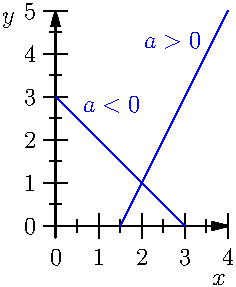
\includegraphics{rechten.pdf}
    \end{center}
    Als $a>0$, is de rechte stijgend.\newline
    Als $a<0$, is de rechte dalend.\newline
    Het snijpunt met de $X$-as is $(-\ds\Frac{b}{a}, 0)$ en met de $Y$-as $(0, b)$
  \item \textcolor{green}{Formules.}\newline
    Indien twee punten van de rechte $(x_1, y_1)$ en $(x_2, y_2)$ gegeven zijn, is de {\bf richtingsco\"effici\"ent}:
    \[a=\ds\Frac{y_2-y_1}{x_2-x_1}\]
    De \hypertarget{vgl_rechte}{vergelijking van de rechte} is dan:
    \[
      y-y_1=a(x-x_1)
    \]\label{vgl_rechte}
  \item \textcolor{green}{Tekenverloop.}\newline
    \begin{tabular}{c|ccccc}
    $x$ & $-\infty$ & & $-\ds\Frac{b}{a}$ & & $+\infty$\\
    \hline
    $ax+b$ & & tegengesteld teken van $a$ & 0 & teken van $a$ & \\		
    \end{tabular}
\end{itemize}

\hypertarget{tweedegraadsfuncties}{}
\subsubsection{Tweedegraadsfuncties} \label{tweedegraadsfuncties}
		\begin{itemize}%tweedegraadsfuncties
		\item \textcolor{green}{Vorm.}
		\[f: x\mapsto ax^2+bx+c \;\;\;\mbox{met}\: a\neq 0\]
		\item \textcolor{green}{Grafiek.}\newline
		Een \hypertarget{parabool}{{\bf parabool}}, waarbij $a$ de aard van de parabool aangeeft:\label{parabool}\newline
		als $a>0$, dan is de holle kant naar boven (dalparabool)\newline 
		%\docLink[tekening]{dalparabool.jpg}{\includegraphics{tekening.gif}}\newline
                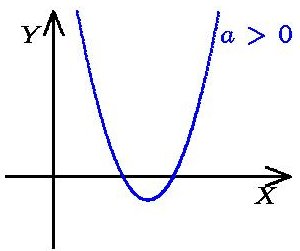
\includegraphics{dalparabool.jpg}
		als $a<0$, dan is de holle kant naar beneden (bergparabool)\newline
		%\docLink[tekening]{bergparabool.jpg}{\includegraphics{tekening.gif}}\newline
                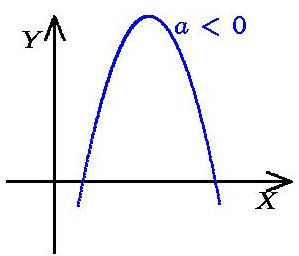
\includegraphics{bergparabool.jpg}
		Verder geldt dat $|a|$ de 'uitrekkingsfactor' voorstelt van de parabool t.o.v. de 		standaardparabool: $P\:\leftrightarrow\: y=x^2$.
		\item \textcolor{green}{Formules.}\newline
		De \hypertarget{topvergelijking}{{\bf top} van de parabool} wordt gegeven door:\label{topvergelijking}
		\[t\:(-\ds\Frac{b}{2a},\ds\Frac{4ac-b^2}{4a}) \]
		en de {\bf symmetrie-as}:
		\[S\:\leftrightarrow\:x=-\ds\Frac{b}{2a}\]
		De {\bf topvergelijking} van de parabool met top $t\:(\alpha, \beta)$
		\[P\:\leftrightarrow\: y=a(x-\alpha)^2+\beta\]
		%\docLink[tekening]{parabool.jpg}{\includegraphics{tekening.gif}}\newline
                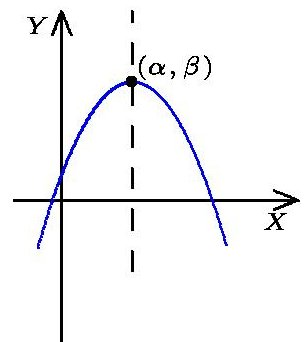
\includegraphics{parabool.jpg}
		\item \textcolor{green}{Tekenverloop.}\newline
		Stel $x_i$ de eventuele nulpunten van de functie $f:x\:\mapsto \:ax^2+bx+c$. 
		De discriminant wordt gegegeven door volgende formule: 
		\[b^2-4ac\]
		en de nulpunten zijn dan
		\[x_{1, 2}=\displaystyle\Frac{-b\pm\sqrt{b^2-4ac}}{2a}\]
		\begin{itemize}%tekenverloop
		\item[*] Discriminant  $>0$\vskip 0.5cm
		\begin{tabular}{c|ccccccc}
		$x$ & $-\infty$ & & $x_1$ & & $x_2$ & & $+\infty$\\
		\hline
		$ax^2+bx+c$ & & teken van $a$ & 0& tegengesteld teken van $a$ & 0 & teken van $a$ 		&\\ 	
		\end{tabular}\vskip 1cm
		\item[*] Discriminant $=0$\vskip 0.5cm
		\begin{tabular}{c|ccccc}
		$x$ & $-\infty$ & & $x_1=x_2$ & & $+\infty$\\
		\hline
		$ax^2+bx+c$ & & teken van $a$ & 0 & teken van $a$ & \\		
		\end{tabular}\vskip 1cm
		\item[*] Discriminant $<0$\vskip 0.5cm
		\begin{tabular}{c|ccc}
		$x$ & $-\infty$ &  & $+\infty$\\
		\hline
		$ax^2+bx+c$ & & teken van $a$ & \\		
		\end{tabular}
		\end{itemize}%tekenverloop
		\end{itemize}%tweedegraadsfuncties

\hypertarget{veeltermfuncties}{}
\subsubsection{Veeltermfuncties} \label{veeltermfuncties}
		\begin{itemize}%veeltermfuncties
		\item \textcolor{green}{Vorm.}
		\[f:x\, \mapsto \: a_nx^n+a_{n-1}x^{n-1}+\ldots +a_1x+a_0\:\mbox{met} \:a_n\neq 0\]
		\item \textcolor{green}{Formules.}\newline
		\hypertarget{euclidische_deling}{{\bf Euclidische deling:}}\label{euclidische_deling} zij $f(x), d(x) \neq 0 \in\R 		[x]$ dan bestaat er juist \'e\'en $q(x)$ en $r(x) \in\R [x]$ zodat geldt:
		 \[f(x)=d(x)\cdot q(x)+r(x)\:\:\mbox{met 		graad}(r(x))<\:\mbox{graad}(d(x))\:\mbox{of}\:r(x)=0\]\newline
		{\bf Praktisch voorbeeld}\newline
		%\docLink[tekening]{euclid.jpg}{\includegraphics{tekening.gif}}\newline
                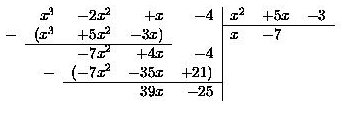
\includegraphics{euclid.jpg}

		\hypertarget{reststelling}{{\bf Reststelling:}}\label{reststelling} De rest van een deling van $f(x)$ door $x-a$ 		is gelijk aan $f(a)$\newline\newline
		{\bf Criterium van deelbaarheid:} \[x-a \: |\: f(x)\:\Leftrightarrow\: f(a)=0\]
		\hypertarget{merkwaardige_quotienten}{{\bf Enkele stellingen:}}\label{merkwaardige_quotienten} 
		\begin{itemize}
		\item[*]Het verschil van twee gelijknamige machten is deelbaar door het verschil van 		de grondtallen.
		\[x^n-a^n=(x-a)(x^{n-1}+ax^{n-2}+a^2x^{n-3}+\ldots+a^{n-2}x+a^{n-1})\]
		\item[*]De som van twee gelijknamige {\it oneven} machten is deelbaar door de som 		van de grondtallen.
		\[x^{2n+1}+a^{2n+1}=(x+a)(x^{2n}-ax^{2n-1}+a^2x^{2n-2}-\ldots-a^{2n-1}x+a^{2n})\]
		\end{itemize}
		{\bf Methode van Horner:} zie %\docLink[formularium]{form_algebra.tex}[n-de graadsvergelijkingen]{$n$-de graadsvergelijkingen}
		\end{itemize}%veeltermfuncties

\hypertarget{rationale_functies}{}
\subsubsection{Gebroken rationale functies} \label{rationale_functies}
			\begin{itemize}%gebroken rationale functies
			\item\textcolor{green}{Vorm.}\newline
			\[f:x\mapsto \ds\Frac{g(x)}{h(x)} \:\mbox{met g(x) en h(x) veeltermen 			en graad}(h(x))\geq 1\]
			\item \textcolor{green}{Kenmerken.}\newline
				\begin{itemize}
				\item[*] domein: $\:\R \backslash h^{-1}\{0\}$
				\item[*] $f^{-1}\{0\}=g^{-1}\{0\}\cap \:\mbox{domein}\:f$
				\end{itemize} 
			\end{itemize}%gebroken rationale functies

\hypertarget{goniometrische_functies}{}
\subsubsection{Goniometrische functies} \label{goniometrische_functies}

\begin{itemize}
\item \textcolor{green}{\hypertarget{periodieke_functies}{Periodieke functies}}\label{periodieke_functies}\newline
Een functie is een {\bf periodieke functie} als en slechts als er een getal $\omega \in \R_0$ bestaat zodat \[\forall x \in \:\mbox{dom}f : f(x+\omega)=f(x).\]
Het kleinste positief getal $\omega$ waarvoor dit geldt, noemen we de {\bf periode} van de functie. Als $m$ en $M$ de kleinste en de grootste functiewaarden zijn die $f$ bereikt, dan noemen we de rechte $y=\frac{m+M}{2}$ de {\bf evenwichtslijn} van de grafiek van $f$. De {\bf amplitude} is de waarde vanaf de evenwichtslijn tot aan de maximale uitwijking.
\item \textcolor{green}{Elementaire goniometrische functies}\newline\newline
\hypertarget{sinusfunctie}{{\bf De sinusfunctie: }}\label{sinusfunctie}$f :x\mapsto\sin x$\vskip 0.5cm

Kenmerken: \begin{itemize}
		\item[*] domein: $\R$
		\item[*] bereik: $[-1, 1]$
		\item[*] $f^{-1}\{0\}=\{k\pi\:|\:k\in\Z\}$
		\item[*] periode: $2\pi$
		\item[*] grafiek %\docLink[tekening]{sinus.jpg}{\includegraphics{tekening.gif}}\newline
                         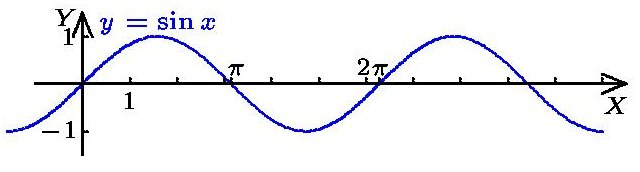
\includegraphics{sinus.jpg}
		\end{itemize}
\hypertarget{cosinusfunctie}{{\bf De cosinusfunctie: }}\label{cosinusfunctie}$f :x\mapsto\cos x$\vskip 0.5cm

Kenmerken: \begin{itemize}
		\item[*] domein: $\R$
		\item[*] bereik: $[-1, 1]$
		\item[*] $f^{-1}\{0\}=\{(2k+1)\ds\Frac{\pi}{2}\:|\:k\in\Z\}$
		\item[*] periode: $2\pi$
		\item[*] grafiek %\docLink[tekening]{cosinus.jpg}{\includegraphics{tekening.gif}}\newline
                         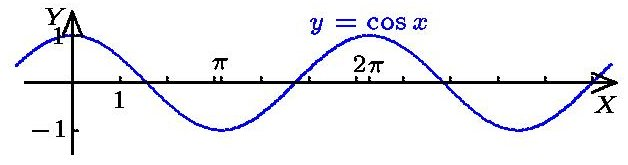
\includegraphics{cosinus.jpg}
		\end{itemize}
\hypertarget{tangensfunctie}{{\bf De tangensfunctie: }}\label{tangensfunctie}$f :x\mapsto\tan{x}$\vskip 		0.5cm
Kenmerken:\begin{itemize}
		\item[*] domein: $\R \backslash \{(2k+1)\ds\Frac{\pi}{2}\:|\:k\in\Z\}$
		\item[*] bereik: $\R$
		\item[*] $f^{-1}\{0\}=\{k\pi\:|\:k\in\Z\}$
		\item[*] periode: $\pi$
		\item[*] grafiek 
		\end{itemize}
		%\docLink[tekening]{tangens.jpg}{\includegraphics{tekening.gif}}\newline
                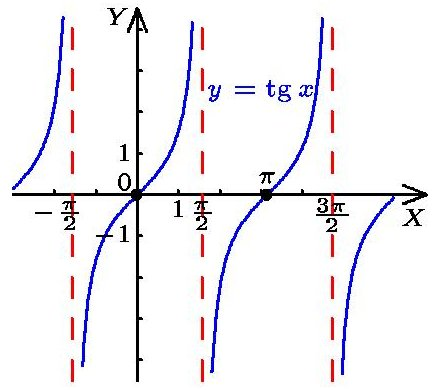
\includegraphics{tangens.jpg}

\hypertarget{}{{\bf De cotangensfunctie: }}\label{cotangensfunctie}$f :x\mapsto\mbox{cotg}x$
\vskip 0.5cm
Kenmerken:\begin{itemize}
		\item[*] domein: $\R \backslash \{k \pi\:|\:k\in\Z\}$
		\item[*] bereik: $\R$
		\item[*] $f^{-1}\{0\}=\{(2k+1)\ds\Frac{\pi}{2}\:|\:k\in\Z\}$
		\item[*] periode: $\pi$
		\end{itemize}	

\item \textcolor{green}{\hypertarget{algemene_sinusfunctie}{Algemene sinusfuncties: }}$f:x\:\mapsto\: a\sin(b(x-c))+d$ \label{algemene_sinusfunctie}\newline\newline
Kenmerken:\begin{itemize}
		\item[*] $|a|$ is de amplitude (maximale uitwijking t.o.v. de 				evenwichtsstand)
		\item[*] periode: $\ds\Frac{2\pi}{b}$
		\item[*] domein: $\R$
		\item[*] bereik: $[-|a|+d, |a|+d]$
		\item[*] $c:$ verschuiving in de richting van de $X$-as over $|c|$ 					\'e\'enheden:\newline
			\begin{itemize}
			\item[*] naar rechts: als $c$ positief is
			\item[*] naar links: als $c$ negatief is
			\end{itemize}
		\item[*] $d:$ verschuiving in de richting van de $Y$-as over $|d|$ 					\'e\'enheden:\newline
			\begin{itemize}
			\item[*] naar boven: als $d$ positief is
			\item[*] naar onder: als $d$ negatief is
			\end{itemize}

		\end{itemize}
\item \textcolor{green}{Toepassing: } $f:x\:\mapsto\:a\sin x+b \cos x$
\newline\newline
Methode voor het omvormen tot een algemene sinusfunctie:
\begin{eqnarray*}
f(x) & = & a\sin{x} + b\cos{x}\\
     & = & a(\sin{x} + \frac{b}{a}\cos{x})\\
     &   & \text{Stel } \ds\Frac{b}{a} = \tan{\varphi}\:\text{ met } \:\varphi \in ]0, \ds\Frac{\pi}{2}[ \:\text{ als }\: \ds\Frac{b}{a} > 0 \\
   %  &   & \hskip 1cm \mbox{Stel } $\:\ds\Frac{b}{a}=$tg$\varphi\:\mbox{ met } \:\varphi \in ]0, \ds\Frac{\pi}{2}[ \:\mbox{ als }\: \ds\Frac{b}{a} > 0$  				\\
     &   & \text{en } \varphi \in ]-\ds\Frac{\pi}{2}, 0[ \:\text{ als }\: \ds\Frac{b}{a} < 0 \\
   %  &   & \hskip 4.3 cm $\varphi \in ]-\ds\Frac{\pi}{2}, 0[ \:\mbox{ als }\: \ds\Frac{b}{a} < 0$  \\
     & = & a(\sin{x} + \tan{\varphi}\cos{x})\\
     & = & a(\sin{x} + \frac{\sin{\varphi}}{\cos{\varphi}}\cos{x})\\
     & = & \ds \Frac{a}{\cos\varphi}(\sin x\ \cos \varphi + \sin \varphi \cos{x})\\			
     & = & \ds \Frac{a}{\cos\varphi}\sin(x + \varphi)
\end{eqnarray*}
	\item \textcolor{green}{Formules}\newline 
%Zie \docLink[formularium]{form_goniometrie.tex}[]{Goniometrie.}
\end{itemize}

\hypertarget{exponentiele_functies}{}
\subsubsection{Exponenti\"ele functies} \label{exponentiele functies}
		\begin{itemize}%exponentiele functies
		\item \textcolor{green}{Vorm}\newline
		\[f: x \mapsto a^x \:\mbox{met}\: a\in \R^+_0\backslash \{1\}\]
		\item \textcolor{green}{Kenmerken}
			\begin{itemize}
			\item[*] domein: $\R$
			\item[*] bereik: $\R^+_0$
			\item[*] $f^{-1}\{0\} = \emptyset$
			\end{itemize}
		\item \textcolor{green}{Speciaal geval}\newline
		\[f: x \mapsto e^x \:\mbox{met $e$ het getal van Euler ($e$ = 		2,718281828459$\ldots$)}\]
		\item \textcolor{green}{Grafiek}\newline
		%\docLink[tekening]{exponentieleB.jpg}{\includegraphics{tekening.gif}}
		%\docLink[tekening]{exponentieleA.jpg}{\includegraphics{tekening.gif}}
                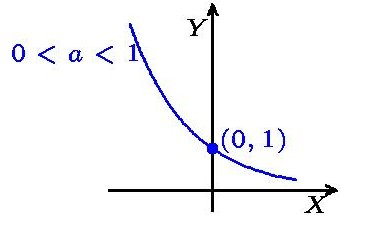
\includegraphics{exponentieleB.jpg}
                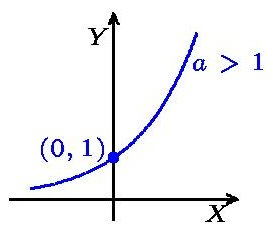
\includegraphics{exponentieleA.jpg}
		\end{itemize}%exponentiele functies

\hypertarget{logaritmische_functies}{}
\subsubsection{Logaritmische functies} \label{logaritmische functies}
		\begin{itemize}%logaritmische functies
		\item  \textcolor{green}{Definitie logaritmen}\newline
		\[\forall a\in \R^+_0\backslash \{1\} : y = \mbox{log}_a x\: \Leftrightarrow\: a^y = 		x\]
		\item \textcolor{green}{Speciale gevallen}\newline
		Briggse logaritme : log $x$ is de logaritme met grondtal $a=10$\newline
		Neperiaanse logaritme: ln $x$ is de logaritme met grondtal $a=e$\newline
		\item \textcolor{green}{Vorm}
		\[f:x\mapsto \mbox{log}_a x \: \mbox{met}\: a\in \R^+_0\backslash \{1\}\]
		\item \textcolor{green}{Kenmerken}
			\begin{itemize}
			\item[*] domein: $\R^+_0$
			\item[*] bereik: $\R$
			\item[*] $f^{-1}\{0\} = \{1\}$
			\end{itemize}
		\item \textcolor{green}{Grafiek}\newline
		%\docLink[tekening]{logaritmischeB.jpg}{\includegraphics{tekening.gif}}
		%\docLink[tekening]{logaritmischeA.jpg}{\includegraphics{tekening.gif}}
                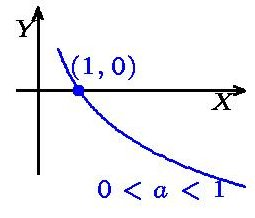
\includegraphics{logaritmischeB.jpg}
                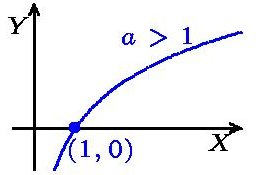
\includegraphics{logaritmischeA.jpg}
		\item \textcolor{green}{\hypertarget{logaritmen}{Formules}}\label{logaritmen}\newline
			\begin{itemize}
			\item[*] Gevolg van de definitie:
			\[\mbox{log}_a \:a^y =y\:\: \mbox{ en }\:\: a^{\mbox{log}_a \:x}=x\]
			\item[*] Logaritme van een product.
			\[\forall x_1, x_2, x_3 \in \R^+_0 : \mbox{log}_a\:(x_1 \cdot x_2\cdot x_3) = 			\mbox{log}_a \:x_1 + \mbox{log}_a \:x_2 + \mbox{log}_a \:x_3 \]
			\item[*] Logaritme van een quoti\"ent.
			\[\forall x_1, x_2 \in \R^+_0 : \mbox{log}_a\:(\ds\Frac {x_1}{x_2}) = 			\mbox{log}_a \:x_1 - \mbox{log}_a \:x_2 \]
			\item[*] Logaritme van een macht.
			\[\forall x \in \R^+_0\:;\: \forall r \in \R \: : \:\mbox{log}_a \:x^r 			= r\:\mbox{log}_a \:x\]
			\item[*] Verandering van grondtal.
			\[\mbox{log}_b \:x =\ds\Frac{\mbox{log}_a\:x}{\mbox{log}_a \:b}\]
			\end{itemize}
		 
		\end{itemize}%logaritmische functies


\hypertarget{bijzondere_functies}{}
\subsubsection{Grafieken van enkele bijzondere functies} \label{bijzondere_functies}

\begin{itemize}
\item[*] \textcolor{green}{\hypertarget{absolute_waardefunctie}{Absolute waardefunctie: $y=|\,x\,|$}} \label{absolute_waardefunctie}
  \begin{center}
  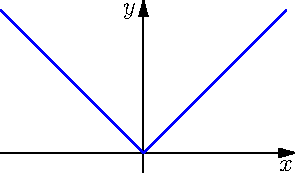
\includegraphics{absolute_waarde}
  \end{center}
\item[*] \textcolor{green}{Geheelfunctie (\hypertarget{trapfunctie}{trapfunctie}): $y=\lfloor\,x\,\rfloor$} \label{trapfunctie}\newline
  Dit is een functie waarbij $\lfloor\,x\,\rfloor$ het grootste geheel getal voorstelt kleiner dan of gelijk aan $x$.
  \begin{center}
  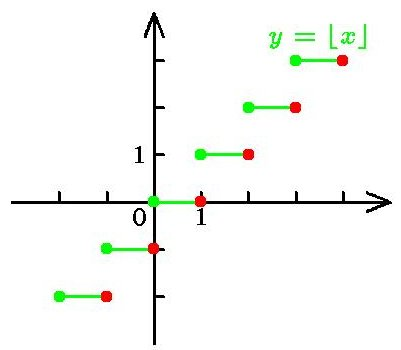
\includegraphics{trap.jpg}
  \end{center}
\item[*] \textcolor{green}{De functie \hypertarget{vierkantswortel}{$y=\sqrt{x}$}} \label{vierkantswortel}
  \begin{center}
  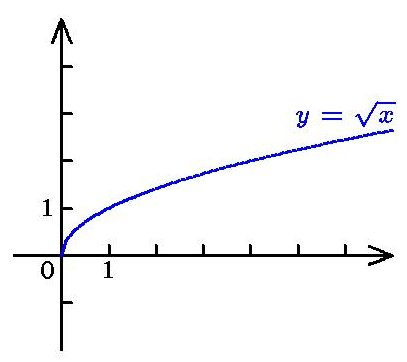
\includegraphics{vierkantswortel.jpg}
  \end{center}
\end{itemize}


% Dit werk is gelicenseerd onder een Creative Commons
% Naamsvermelding-GelijkDelen 3.0 Unported.
% Bezoek http://creativecommons.org/licenses/by-sa/3.0/ om een kopie te zien 
% van de licentie of stuur een brief naar Creative Commons, 444 Castro Street, 
% Suite 900, Mountain View, California, 94041, USA.
